\documentclass[a4paper,12pt]{article}
\usepackage[english,ukrainian,russian]{babel}
\linespread{1}
\usepackage{ucs}
\usepackage[utf8]{inputenc}
\usepackage[T2A]{fontenc}
\usepackage[paper=portrait,pagesize]{typearea}
\usepackage{amsmath}
\usepackage{bigints}
\usepackage{amsfonts}
\usepackage{graphicx}
\usepackage{amssymb}
\usepackage{cancel}
\usepackage{gensymb}
\usepackage{multirow}
\usepackage{rotate} 
\usepackage{pdflscape}
\usepackage{bigstrut}
\usepackage[pageanchor]{hyperref}
\usepackage{chngpage}
\usepackage{fancybox,fancyhdr}
\newcommand\tab[1][1cm]{\hspace*{#1}}
\newcommand{\RomanNumeralCaps}[1]{\MakeUppercase{\romannumeral #1}}
\usepackage[left=20mm, top=20mm, right=15mm, bottom=15mm, nofoot]{geometry}


\begin{document}
    \pagestyle{fancy}
    \fancyhead{}
    \fancyhead[R]{ФІ-12 Завалій Олександр}
    \begin{center}
        \large{\textbf{Міністерство освіти і науки України\\
                Національний технічний університет України\\
                «Київський політехнічний інститут імені Ігоря Сікорського»\\
                Навчально-науковий Фізико-технічний інститут}}\\
        \hfill \break \hfill \break \hfill\break \hfill \break \hfill \break \hfill \break \hfill \break
        \hfill \break \hfill \break \hfill \break
        \begin{center}
            \normalsize{\textbf{ОПЕРАЦІЙНІ СИСТЕМИ\\
            Комп’ютерний практикум\\
            Робота №2}}
        \end{center}
    \end{center}
    \hfill \break \hfill \break \hfill \break \hfill \break \hfill \break \hfill \break \hfill \break
    \hfill \break \hfill \break \hfill \break \hfill \break 
    \begin{flushright}
        \large{ \hspace{35pt} Виконав:\\
            студент групи ФI-12\\
            Завалій Олександр\\} 
        \large{ \hspace{35pt} Перевірив:\\
        Кірієнко О.В.} 
    \end{flushright}
    \hfill \break \hfill \break \hfill \break \hfill \break \hfill \break \hfill \break \hfill \break
    \hfill \break
    \begin{center} \textbf{Київ-2023} \end{center}
    \thispagestyle{empty}

\newpage
    \begin{center}
        \section*{\bfseries{Робота №2.\\
        Система розмежування доступу в UNIX і
        Linux, права доступу до файлів і керування ними}}
    \end{center}
    \textbf{Мета:} \\
    \hangindent=1.5cm 
    \hangafter=+1 \noindent
    Оволодіння практичними навичками керування
    правами доступу до файлів і їхній аналіз в ОС UNIX та
    Linux \\
    \begin{center}
        \Large{Варіант №5}
    \end{center}
    Зміст індивідуального завдання:
    \begin{enumerate}
        \item Створіть каталог \textbf{lab\_2}.
        \item Скопіюйте в каталог \textbf{lab\_2} файл \textbf{/bin/cat} під назвою \textbf{my\_cat}.
        \item За допомогою файлу \textbf{my\_cat}, що знаходиться в каталозі \textbf{lab\_2}, перегляньте уміст файлу \textbf{.profile} (ви знаходитесь у домашньому каталозі).
        \item Перегляньте список файлів у каталозі \textbf{lab\_2}. Потім перегляньте список усіх файлів, включаючи приховані, з
        повною інформацією про файли. Зверніть увагу на права доступу, власника, дату модифікації файлу, що ви тількино скопіювали. 
        Потім перегляньте цю інформацію про оригінальний файл (той, який копіювали) і порівняйте два результати.
        \item Змініть права доступу до файлу \textbf{my\_cat} так, щоб власник міг тільки читати цей файл.
        \item Переконайтеся в тому, що ви зробили ці зміни і повторіть п.3.
        \item Визначте права на файл \textbf{my\_cat} таким чином, щоб ви могли робити з файлом усе, що завгодно, а всі інші — нічого не могли робити.
        \item Поверніться в домашній каталог. Змініть права доступу до каталогу \textbf{lab\_2} так, щоб ви могли його тільки читати.
        \item Спробуйте переглянути простий список файлів у цьому каталозі. Спробуйте переглянути список файлів з повною інформацією про них. Спробуйте запустити і видалити
        файл \textbf{my\_cat} з цього каталогу.
        \item Поясніть отримані результати. Результати виконання п.8 можуть бути різними в різних версіях UNIX, зокрема, Linux і FreeBSD. Прокоментуйте отримані результати у
        висновках.
        \item За допомогою команди \textbf{su <user name>}, завантажтесь в систему, користуючись обліковим записом іншого користувача. (Вам потрібно знати пароль цього
        користувача.) Спробуйте отримати доступ до Вашого каталогу \textbf{lab\_2}. Перевірте, чи правильно зроблено завдання попереднього пункту. Створіть каталог \textbf{lab\_2\_2}.
        \item Знову завантажтесь в систему, користуючись своїм обліковим записом. Спробуйте зробити власником каталогу \textbf{lab\_2} іншого користувача. Спробуйте зробити 
        себе власником каталогу \textbf{lab\_2\_2}. Поясніть результати.
        \item Зайдіть у каталог \textbf{lab\_2}. Зробіть так, щоб нові створені файли і каталоги діставали права доступу згідно Таблиці. Створіть новий файл і каталог і переконайтеся в
        правильності ваших установок. Права для файлів \textbf{<<644>>}. Права для каталогів \textbf{<<745>>}.
    \end{enumerate}

\newpage
    \begin{enumerate}
    \item[14.] Поверніть собі права читати, писати, та переглядати вміст каталогів.
    \item[15.] Створіть у каталозі \textbf{lab\_2} каталог \textbf{acl\_test} та у ньому файли \textbf{file1}, \textbf{file2}. Після створення \textbf{file1} додайте у 
    нього довільний текст.
    \item[16.] Виведіть ACL для \textbf{file1}.
    \item[17.] Змінить права доступу на \textbf{file1} так, щоб тільки власник мав право на читання.
    \item[18.] Увійдіть до системи під іншим обліковим записом та спробуйте прочитати вміст \textbf{file1}. Що отримаємо? Поверніться до свого облікового запису.
    \item[19.] За допомогою команди \textbf{setfacl} додайте право на читання іншому обраному користувачу для \textbf{file1}. Перевірте, що створився новий ACL для \textbf{file1}.
    \item[20.] Увійдіть до системи під іншим обліковим записом та спробуйте прочитати вміст \textbf{file1}. Що отримаємо? Поверніться до свого облікового запису.
    \item[21.] За допомогою команди \textbf{setfacl} встановіть значення маски таким чином щоб дозволити читати вміст \textbf{file1} іншому користувачу. Виведіть ACL для \textbf{file1}.
    \item[22.] Увійдіть до системи під іншим обліковим записом, та спробуйте прочитати вміст \textbf{file1}. Ви повинні мати таку змогу.
    \end{enumerate}

\newpage
    \begin{center}
        \Large{Task \RomanNumeralCaps{1}}
    \end{center}
    Створіть каталог \textbf{lab\_2}.
    \begin{figure}[h!]
        \begin{minipage}[h]{1\linewidth}
            \centering
            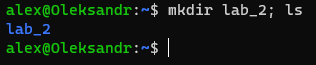
\includegraphics[width=0.5\linewidth]{Prt sc/Figure_1.png}  
        \end{minipage}
    \end{figure}

    \begin{center}
        \Large{Task \RomanNumeralCaps{2}}
    \end{center}
    Скопіюйте в каталог \textbf{lab\_2} файл \textbf{/bin/cat} під назвою \textbf{my\_cat}.
    \begin{figure}[h!]
        \begin{minipage}[h]{1\linewidth}
            \centering
            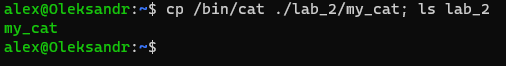
\includegraphics[width=0.6\linewidth]{Prt sc/Figure_2.png}  
        \end{minipage}
    \end{figure}

    \begin{center}
        \Large{Task \RomanNumeralCaps{3}}
    \end{center}
    За допомогою файлу \textbf{my\_cat}, що знаходиться в каталозі \textbf{lab\_2}, перегляньте уміст файлу \textbf{.profile} (ви знаходитесь у домашньому каталозі).
    \begin{figure}[h!]
        \begin{minipage}[h]{1\linewidth}
            \centering
            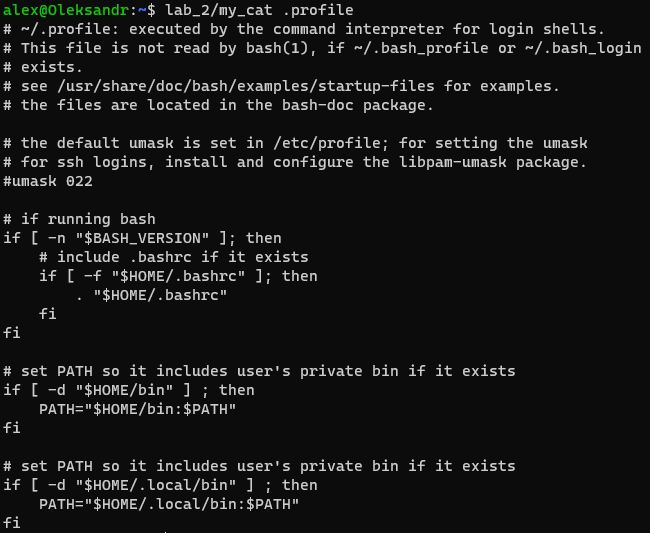
\includegraphics[width=0.7\linewidth]{Prt sc/Figure_3.png}  
        \end{minipage}
    \end{figure}

\newpage
    \begin{center}
        \Large{Task \RomanNumeralCaps{4}}
    \end{center}
    Перегляньте список файлів у каталозі \textbf{lab\_2}. Потім перегляньте список усіх файлів, включаючи приховані, з
    повною інформацією про файли. Зверніть увагу на права доступу, власника, дату модифікації файлу, що ви тількино скопіювали. 
    Потім перегляньте цю інформацію про оригінальний файл (той, який копіювали) і порівняйте два результати.
    \begin{figure}[h!]
        \begin{minipage}[h]{1\linewidth}
            \centering
            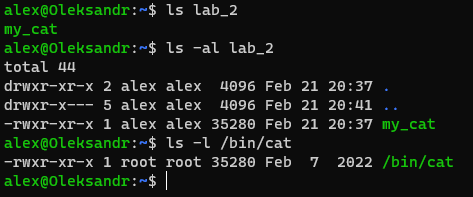
\includegraphics[width=0.6\linewidth]{Prt sc/Figure_4.png}  
        \end{minipage}
    \end{figure}

    \begin{center}
        \Large{Task \RomanNumeralCaps{5}}
    \end{center}
    Змініть права доступу до файлу \textbf{my\_cat} так, щоб власник міг тільки читати цей файл.
    \begin{figure}[h!]
        \begin{minipage}[h]{1\linewidth}
            \centering
            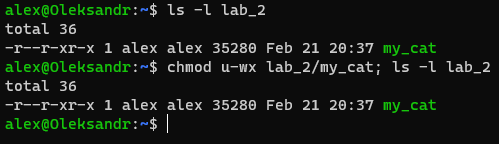
\includegraphics[width=0.6\linewidth]{Prt sc/Figure_5.png}  
        \end{minipage}
    \end{figure}

    \begin{center}
        \Large{Task \RomanNumeralCaps{6}}
    \end{center}
    Переконайтеся в тому, що ви зробили ці зміни і повторіть п.3.
    \begin{figure}[h!]
        \begin{minipage}[h]{1\linewidth}
            \centering
            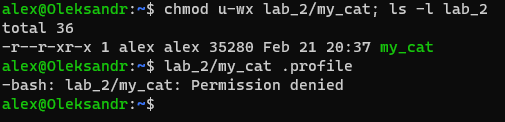
\includegraphics[width=0.6\linewidth]{Prt sc/Figure_6.png}  
        \end{minipage}
    \end{figure}

    \begin{center}
        \Large{Task \RomanNumeralCaps{7}}
    \end{center}
    Визначте права на файл \textbf{my\_cat} таким чином, щоб ви могли робити з файлом усе, що завгодно, а всі інші — нічого не могли робити.
    \begin{figure}[h!]
        \begin{minipage}[h]{1\linewidth}
            \centering
            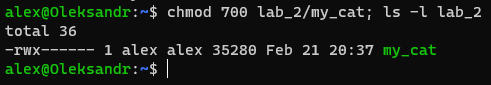
\includegraphics[width=0.6\linewidth]{Prt sc/Figure_7.png}  
        \end{minipage}
    \end{figure}

\newpage
    \begin{center}
        \Large{Task \RomanNumeralCaps{8}}
    \end{center}
    Поверніться в домашній каталог. Змініть права доступу до каталогу \textbf{lab\_2} так, щоб ви могли його тільки читати.
    \begin{figure}[h!]
        \begin{minipage}[h]{1\linewidth}
            \centering
            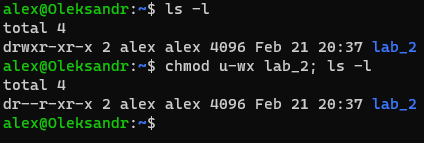
\includegraphics[width=0.6\linewidth]{Prt sc/Figure_8.png}  
        \end{minipage}
    \end{figure}

    \begin{center}
        \Large{Task \RomanNumeralCaps{9}}
    \end{center}
    Спробуйте переглянути простий список файлів у цьому каталозі. Спробуйте переглянути список файлів з повною інформацією про них. Спробуйте запустити і видалити
    файл \textbf{my\_cat} з цього каталогу.
    \begin{figure}[h!]
        \begin{minipage}[h]{1\linewidth}
            \centering
            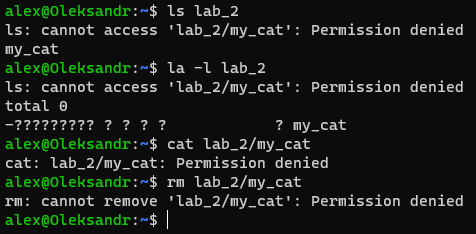
\includegraphics[width=0.6\linewidth]{Prt sc/Figure_9.png}  
        \end{minipage}
    \end{figure}

    \begin{center}
        \Large{Task \RomanNumeralCaps{10}}
    \end{center}
    Поясніть отримані результати. Результати виконання п.8 можуть бути різними в різних версіях UNIX, зокрема, Linux і FreeBSD. Прокоментуйте отримані результати у
    висновках. \\
    Оскільки ми встановили права доступу для власника тільки на читання. Ми можемо переглядати(читати) вміст каталогу. 
    Відповідно до логіки роботи ми не можемо виконувати запис та виконня для всього дерева цієї директорії.
    
\newpage
    \begin{center}
        \Large{Task \RomanNumeralCaps{11}}
    \end{center}
    За допомогою команди \textbf{su <user name>}, завантажтесь в систему, користуючись обліковим записом іншого користувача. (Вам потрібно знати пароль цього
    користувача.) Спробуйте отримати доступ до Вашого каталогу \textbf{lab\_2}. Перевірте, чи правильно зроблено завдання попереднього пункту. Створіть каталог \textbf{lab\_2\_2}.
    \begin{figure}[h!]
        \begin{minipage}[h]{1\linewidth}
            \centering
            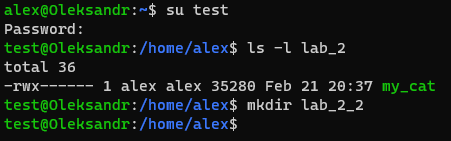
\includegraphics[width=0.6\linewidth]{Prt sc/Figure_11.png}  
        \end{minipage}
    \end{figure}

    \begin{center}
        \Large{Task \RomanNumeralCaps{12}}
    \end{center}
    Знову завантажтесь в систему, користуючись своїм обліковим записом. Спробуйте зробити власником каталогу \textbf{lab\_2} іншого користувача. Спробуйте зробити 
    себе власником каталогу \textbf{lab\_2\_2}. Поясніть результати.
    \begin{figure}[h!]
        \begin{minipage}[h]{1\linewidth}
            \centering
            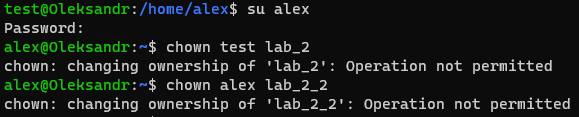
\includegraphics[width=0.6\linewidth]{Prt sc/Figure_12.png}  
        \end{minipage}
    \end{figure} \\
    Основна модель безпеки в Unix стосується користувачів і груп, а також їх права власності на різні файли та каталоги. Це означає, що без 
    підвищених привілеїв (стати root або виконувати команди через sudo) жоден звичайний користувач не матиме достатніх привілеїв, щоб діяти від імені іншого користувача.

    \begin{center}
        \Large{Task \RomanNumeralCaps{13}}
    \end{center}
    Зайдіть у каталог \textbf{lab\_2}. Зробіть так, щоб нові створені файли і каталоги діставали права доступу згідно Таблиці. Створіть новий файл і каталог і переконайтеся в
    правильності ваших установок. Права для файлів \textbf{<<644>>}. Права для каталогів \textbf{<<745>>}.
    \begin{figure}[h!]
        \begin{minipage}[h]{1\linewidth}
            \centering
            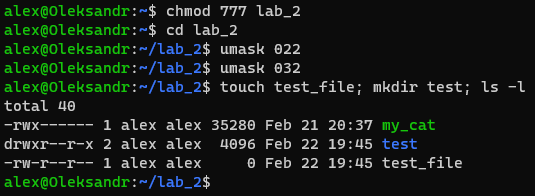
\includegraphics[width=0.6\linewidth]{Prt sc/Figure_13.png}  
        \end{minipage}
    \end{figure}

\newpage
    \begin{center}
        \Large{Task \RomanNumeralCaps{14}}
    \end{center}
    Поверніть собі права читати, писати, та переглядати вміст каталогів.
    \begin{figure}[h!]
        \begin{minipage}[h]{1\linewidth}
            \centering
            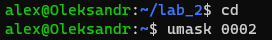
\includegraphics[width=0.6\linewidth]{Prt sc/Figure_14.png}  
        \end{minipage}
    \end{figure}

    \begin{center}
        \Large{Task \RomanNumeralCaps{15}}
    \end{center}
    Створіть у каталозі \textbf{lab\_2} каталог \textbf{acl\_test} та у ньому файли \textbf{file1}, \textbf{file2}. Після створення \textbf{file1} додайте у 
    нього довільний текст.
    \begin{figure}[h!]
        \begin{minipage}[h]{1\linewidth}
            \centering
            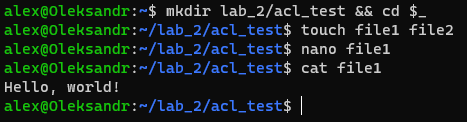
\includegraphics[width=0.6\linewidth]{Prt sc/Figure_15.png}  
        \end{minipage}
    \end{figure}

    \begin{center}
        \Large{Task \RomanNumeralCaps{16}}
    \end{center}
    Виведіть ACL для \textbf{file1}.
    \begin{figure}[h!]
        \begin{minipage}[h]{1\linewidth}
            \centering
            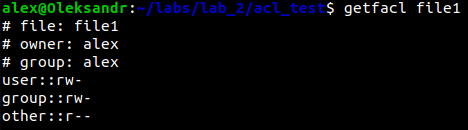
\includegraphics[width=0.6\linewidth]{Prt sc/Figure_16.png}  
        \end{minipage}
    \end{figure}

    \begin{center}
        \Large{Task \RomanNumeralCaps{17}}
    \end{center}
    Змінить права доступу на \textbf{file1} так, щоб тільки власник мав право на читання.
    \begin{figure}[h!]
        \begin{minipage}[h]{1\linewidth}
            \centering
            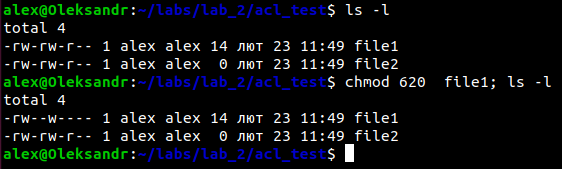
\includegraphics[width=0.6\linewidth]{Prt sc/Figure_17.png}  
        \end{minipage}
    \end{figure}

\newpage
    \begin{center}
        \Large{Task \RomanNumeralCaps{18}}
    \end{center}
    Увійдіть до системи під іншим обліковим записом та спробуйте прочитати вміст \textbf{file1}. Що отримаємо? Поверніться до свого облікового запису.
    \begin{figure}[h!]
        \begin{minipage}[h]{1\linewidth}
            \centering
            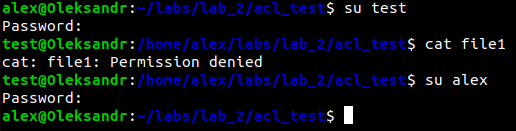
\includegraphics[width=0.6\linewidth]{Prt sc/Figure_18.png}  
        \end{minipage}
    \end{figure}

    \begin{center}
        \Large{Task \RomanNumeralCaps{19}}
    \end{center}
    За допомогою команди \textbf{setfacl} додайте право на читання іншому обраному користувачу для \textbf{file1}. Перевірте, що створився новий ACL для \textbf{file1}.
    \begin{figure}[h!]
        \begin{minipage}[h]{1\linewidth}
            \centering
            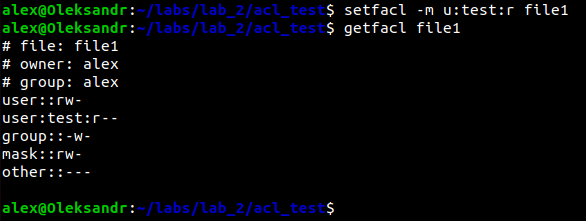
\includegraphics[width=0.6\linewidth]{Prt sc/Figure_19.png}  
    
        \end{minipage}
    \end{figure}

    \begin{center}
        \Large{Task \RomanNumeralCaps{20}}
    \end{center}
    Увійдіть до системи під іншим обліковим записом та спробуйте прочитати вміст \textbf{file1}. Що отримаємо? Поверніться до свого облікового запису.
    \begin{figure}[h!]
        \begin{minipage}[h]{1\linewidth}
            \centering
            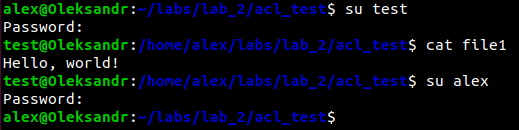
\includegraphics[width=0.6\linewidth]{Prt sc/Figure_20.png}  
        \end{minipage}
    \end{figure}

\newpage
    \begin{center}
        \Large{Task \RomanNumeralCaps{21}}
    \end{center}
    За допомогою команди \textbf{setfacl} встановіть значення маски таким чином щоб дозволити читати вміст \textbf{file1} іншому користувачу. Виведіть ACL для \textbf{file1}.
    \begin{figure}[h!]
        \begin{minipage}[h]{1\linewidth}
            \centering
            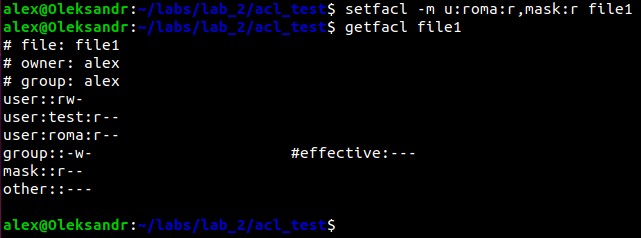
\includegraphics[width=0.6\linewidth]{Prt sc/Figure_21.png}  
        \end{minipage}
    \end{figure}

    \begin{center}
        \Large{Task \RomanNumeralCaps{22}}
    \end{center}
    Увійдіть до системи під іншим обліковим записом, та спробуйте прочитати вміст \textbf{file1}. Ви повинні мати таку змогу.
    \begin{figure}[h!]
        \begin{minipage}[h]{1\linewidth}
            \centering
            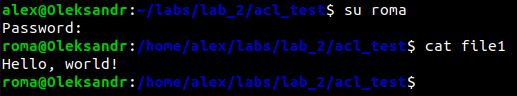
\includegraphics[width=0.6\linewidth]{Prt sc/Figure_22.png}  
        \end{minipage}
    \end{figure}

    \begin{center}
        \Large{Висновки}
    \end{center}
    
    З огляду вивченого матеріалу, використання команд: <<ls –l>>, <<chmod>>, <<chown>>, <<umask>>, <<setfacl>> та <<getfacl>> є незамінною частиною 
    розмежування прав доступу до файлів і керування ними.

    UNIX реалізує дискреційну модель розмежування доступу, тому для кожного файлу визначається, які права мають всі користувачі на доступ до файлу.
    З цього випливає легкість адміністрування і повний контроль доступу до кожного окремого файлу для всіх можливих користувачів. 
    
    Перед встановленням прав доступу потрібно чітко розуміти можливе застосування цього файлу іншими користувачами та вже наявні права доступу.
    Тому, щоб створювати нові файли вже по наявному шаблону можна задати маску для всіх нових файлів та директорій за домопогою команди <<umask>>. 
    Переглняути інформацію з таблиці індексних дескрипторів можна командою <<ls –l>>. 

    В окремих випадках, для вже створеного файлу або директорії, права доступу можна редагувати командою <<chmod>>. 
    Команда <<chown>> змінює власника даного файлу або папки, яким може бути користувач або група. 

    Команда <<setfacl>> в Linux використовується для встановлення списків керування доступом (ACL) до файлів. 
    ACL файлу визначає користувачів і групи, яким дозволено доступ до файлу, а також дозволи, які вони мають. 
    Команду <<setfacl>> можна використовувати для додавання, видалення або зміни ACL файлу. Для перегляду ACL використовують <<getfacl>>.

\end{document}